\documentclass{article}
\usepackage{tikz}
\begin{document}
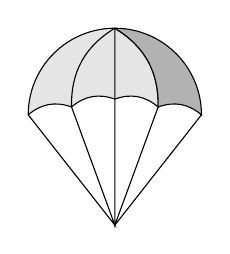
\begin{tikzpicture}
% 伞面最左侧至最右侧
\coordinate (a) at (-1.1cm,0);
\coordinate (b) at (-5.5mm,1mm);
\coordinate (c) at (0,2mm);
\coordinate (d) at (5.5mm,1mm);
\coordinate (e) at (1.1cm,0);
% 伞顶部
\coordinate (f) at (0,1.1cm);
% 伞底部
\coordinate (g) at (0,-1.4cm);
% 伞面
\draw[fill=black!10] (a) to[bend left] (b) to[bend left] (c) to[bend left] (d) to[bend right] (f) arc[start angle=90, end angle=180, radius=1.1cm];
\draw[fill=black!30] (f) to[bend left] (d) to[bend left] (e) arc[start angle=0, delta angle=90, radius=1.1cm];
\draw (c) to (f) to[bend right] (b);
\draw (a) to (g) to (b);
\draw (c) to (g) to (d);
\draw (g) to (e);
\end{tikzpicture}
\end{document}
